\subsection{Descripción del problema.}

\vspace*{0.3cm}

El objetivo de este problema es, \textbf{dado un conjunto de edificios} representados
por la posición de sus paredes izquierda, derecha y su altura, representar el
contorno en el horizonte formado por la superposición de los mismos, \textbf{excluyendo
las líneas internas}.

\vspace*{0.5cm}

\textbf{Ejemplo:}
\begin{itemize}
  \item Para un conjunto de 3 edificios, cuyas coordenadas son (4, 2, 11),
  (5, 4, 7) y (9, 5, 12), donde la primer coordenada es la ubicación de la pared
  izquierda sobre el eje $x$, la segunda coordenada es la altura en el eje $y$ y la
  tercer coordenada es la ubicación de la pared derecha sobre el eje $x$, la
  solución debe ser 4 2 5 4 7 2 9 5 12 0 (es \textbf{única}).

  En la \textbf{figura 5}, que se encuentra debajo, puede visualizarse mejor este ejemplo.
\end{itemize}

\vspace*{0.5cm}

\begin{figure}[h]
  \begin{center}
    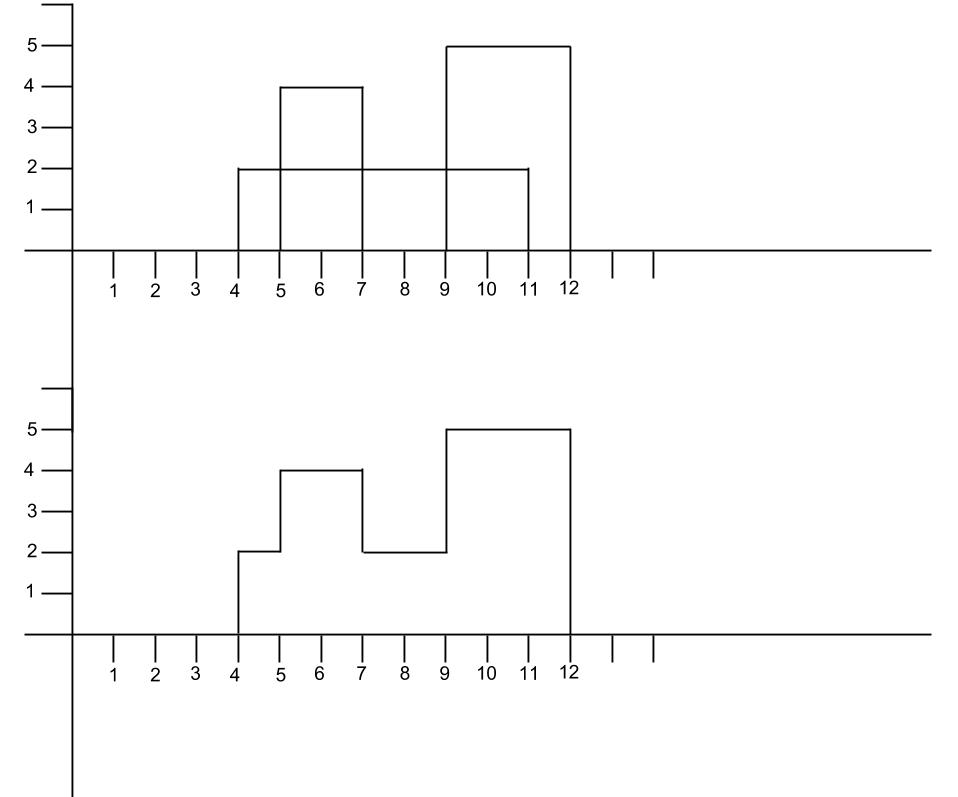
\includegraphics[scale=0.4]{imagenes/ej2.jpg}
  \end{center}
    \caption{ejemplo de puntos de entrada y su correspondiente salida.}
\end{figure}


\newpage


\subsection{Desarrollo de la idea y pseudocódigo.}

\vspace*{0.3cm}

El algoritmo propuesto para resolver este problema consiste en tomar a los edificios
por los 2 vértices que lo identifican (sus puntos con coordenada $y \neq 0$).

\textbf{Recorriendo esos vértices en orden}, los pertenecientes a una pared izquierda
generarán un nuevo punto en el horizonte si son más altos que el último punto agregado
y los que correspondan a una pared derecha, si corresponden al final de la
altura actual, generarán un punto en la intersección con la siguiente altura mayor.

Para saber hasta dónde se debe ''bajar'' luego de un vértice de pared derecha, se
mantiene un \textbf{multiconjunto de alturas}. Cada vértice de pared izquierda carga su
altura y los de pared derecha la eliminan.

\begin{codebox}
\Procname{$\proc{calcularHorizonte}(vertices)$}
\li \Comment vertices: vector de vértices
\li $\id{horizonte} \gets \emptyset$
\li $\id{alturas} \gets \emptyset$
\li $\proc{sort}(vertices)$
\li $\id{vertice} \gets \proc{primero}(vertices)$
\li $\proc{agregar}(horizonte, <vertice.x, vertice.y>)$
\li $\proc{agregar}(alturas, vertice.y)$
\li \While $vertice \neq \proc{ultimo}(vertices)$
      \Do
\li     \If $vertice.posicion_{pared} \isequal izquierda$
          \Then
\li         \If $vertice_y > \proc{ultimo}(horizonte)_y$
              \Then
\li             \If $vertice_x > \proc{ultimo}(horizonte)_x$
                  \Then
\li                 $\proc{agregar}(horizonte, <vertice_x, vertice_y>)$
\li               \Else
\li                 $\proc{ultimo}(horizonte)_y \gets vertice_y$
                 \End
              \End
\li         $\proc{agregar}(alturas, vertice_y)$
\li       \Else
\li         $\proc{quitar}(alturas, vertice_y)$
\li         \If $vertice_y > \proc{maximo}(alturas)$
              \Then
\li             $\proc{agregar}(horizonte, <vertice_x, maximo(alturas)>)$
              \End
          \End
\li     $\id{vertice} \gets \proc{proximo}(vertice)$
      \End
\li \Return $\id{horizonte}$
\end{codebox}



\subsection{Justificación de la resolución y demostración de correctitud.}

\vspace*{0.3cm}


Dado un conjunto de edificios $E$, la solución será un conjunto de puntos
$S_E = \{p \in \mathbb{Z}^2 : \exists e \in E / (p_x = e_i \land p_y = e_y) \land
p \notin T_E\} \cup \{p \in \mathbb{Z}^2 : \exists e \in E / (p_x = e_d \land p
\notin T_E) \land p_y = \max({\{e_y : e \in E \land e_i \leq p_x < e_d\} \cup \{0\}})\}$,
donde $T_E = \{p \in \mathbb{Z}^2 : \exists e \in E / (e_i \leq p_x \leq e_d \land p_y \leq e_y)\}$
son los puntos cubiertos por todos los edificios, donde, dado un edificio
$e$, $e_i$ es el valor en $x$ de su pared izquierda, $e_d$ el valor de su
pared derecha y $e_y$ su altura en $y$, y dado un punto $p \in
\mathbb{Z}^2$, $p_x$ es su coordenada $x$ y $p_y$ su coordenada $y$.

Para demostrar la correctitud de este algoritmo, veremos que cumple con la
definición dada más arriba.

Primero, cada edificio $e_j \in E$ es descompuesto en $p_{j_i} = (e_i, e_y)$ y
$p_{j_d} = (e_d, e_y)$ y se define $P = \bigcup_{j=1}^n \{p_{j_i}, p_{j_d}\}$.
El algoritmo ordena $P$ primero por coordenada $x$ y en caso de empate por
coordenada $y$.

Por cada punto $p \in P$, se revisa si corresponde agregar o modificar un punto
a la solución parcial, de la siguiente manera:

\begin{itemize}
  \item Si es un vértice izquierdo del edificio, $p = (e_i, e_y)$, se carga su
  altura en un multiconjunto $H$ de alturas.
  \begin{itemize}
    \item Si su altura es menor o igual a la del último punto agregado a $H$,
    como vamos recorriendo en orden, podemos asegurar que $\exists e \in E /
    e_i \leq p_x \leq e_d \land p_y \leq e_y$, es decir, $p \in T_E$, por lo
    cual este punto no pertenece a la solución.

    \item Si su altura es mayor a la del último punto agregado a $H$ y también
    lo es su coordenada $x$, entonces podemos asegurar que $\nexists e \in E /
    e_i < p_x \land p_y \leq e_y$, es decir, no está cubierto por un edificio
    que comience antes y por lo tanto, dicho punto es agregado al conjunto
    solución $S$. En el caso de que el último punto agregado a $H$, $h$
    cumpla $h_x = p_x \wedge h_y < p_y \wedge h \in S$, se reemplaza en $S$
    $h$ por $p$.

%    \item Si su altura es mayor a la del último punto y sus coordenadas $X$ son
%    iguales, quiere decir que el punto cargado no estaba cubierto por uno que comience
%    antes, sino por uno que comienza en el mismo punto, pero que es más alto.
%    En este caso reemplazamos la atura cargada en el último punto, por la altura
%    de este.
  \end{itemize}

  \item Si es un vértice derecho del edificio, $p = (e_d, e_y)$, se elimina su
  altura del munticonjunto $H$.
  \begin{itemize}
    \item Si su altura sigue siendo igual a la máxima del multiconjunto, podemos
    afirmar que $\exists e \in E / e_i \leq p_x \leq e_d \land p_y \leq
    e_y$. Es decir, $p \in T_E$ y por lo tanto no corresponde agregarlo a
    $S$.

    \item Si su altura es mayor a la máxima del multiconjunto,
    $\nexists e \in E / e_i < p_x \land p_y \leq e_y$, lo que marca el
    final de un edificio en el horizonte. Por lo tanto se agrega punto $p' =
    (e_d, \max\{h_y : h \in H\} \cup \{0\})$ a $S$.
%    ya que al recorrer en orden, en alturas quedan $\{e_y \in \mathbb{Z} : e \in E / e_i \leq p_x < e_x\}$
  \end{itemize}
\end{itemize}

De esta modo, todos los puntos pertenecientes a $S$ cumplen las mismas
condiciones que los puntos pertenecientes a $S_E$. Por lo tanto, $S
\subseteq S_E$. Pero no existe $s \in S_E$ tal que $s \notin S$, pues eso
diría que $s = (e_d, e_y) \lor s = (e_i, e_y)$ para cierto $e \in E$ y dicho
$e$ fue procesado por nuestro algoritmo y como cumple las condiciones de
$S_E$, $s \in S$. Luego $S = S_E$.


\subsection{Análisis de complejidad.}

\vspace*{0.3cm}

Para el análisis de complejidad nos basaremos en el pseudocódigo de la función
\textsc{calcularHorizonte}, correspondiente al ítem \textbf{4.2}.

\begin{enumerate}
   \item Las siguientes operaciones realizadas sobre el \textit{contenedor} \verb|vector| de la \textit{STL} toman tiempo constante $O(1)$:
<<<<<<< Updated upstream
   \verb|size|, \verb|push_back|, \verb|back|, \verb|empty|, creación y manipulación de iteradores, \verb|begin|, \verb|end|
   y \verb|operator[]|.

   \item La operación \verb|resize| es lineal, $\in O(n)$.

   \item En el \verb|struct Vertice|, el \textit{constructor} y el \verb|operator<| son $O(1)$. También
   tiene complejidad constante el constructor del \verb|struct Punto|.

   \item En las operaciones utilizadas de \verb|multiset|, \verb|insert| y \verb|find| son logarítmicas,
   $\in O(\log n)$, mientras que \verb|erase|, \verb|empty| y \verb|rbegin| son constantes, $\in O(1)$.

   \item Sobre los iteradores, se realizan las operaciones \verb|++| y \verb|*|, ambas
   con complejidad también constante.

   \item Se implementó la función \verb|maximo|, que dado un \verb|multiset|, devuelve
   el mayor de sus elementos ó 0, si el \verb|multiset| está vacío. Dicha función
   tiene complejidad constante, pues \verb|empty| y \verb|rbegin| son constantes, $\in O(1)$.

   \item El algoritmo \verb|sort| de la \textit{STL} utilizado (línea 4) para ordenar los vértices
   por altura, tiene complejidad $O(n \log n)$.

   \item En la línea 8, se itera sobre todos los edificios y se cargan sus 2 vértices. Dentro
   de este ciclo, la asignación resulta constante. Por lo tanto, ejecutar este ciclo
   toma tiempo lineal, $\in O(n)$. Dentro de este ciclo, todas las operaciones realizadas son
   constantes o logarítmicas, por lo tanto están acotadas por $O(n)$.

   \item Las comparaciones y asignaciones realizadas sobre cada vértice, toman tiempo constante,  $\in O(1)$.
=======
   \verb|size|, \verb|push_back|, \verb|back|, \verb|empty|, al igual que la
   creación y manipulación de iteradores, llevada a cabo mediante
   \verb|begin|, \verb|rbegin| \verb|end|, \verb|operator++|,
   \verb|operator*| y \verb|operator[]|.
 
   \item La operación \verb|resize| es lineal, $\in O(n)$.
% 
%   \item En el \verb|struct Vertice|, el \textit{constructor} y el \verb|operator<| son $O(1)$. También
%   tiene complejidad constante el constructor del \verb|struct Punto|.
% 
%   \item En las operaciones utilizadas de \verb|multiset|, \verb|insert| y \verb|find| son logarítmicas, 
%   $\in O(\log n)$, mientras que \verb|erase|, \verb|empty| y \verb|rbegin| son constantes, $\in O(1)$.
% 
%   \item Sobre los iteradores, se realizan las operaciones \verb|++| y \verb|*|, ambas
%   con complejidad también constante.
% 
%   \item Se implementó la función \verb|maximo|, que dado un \verb|multiset|, devuelve
%   el mayor de sus elementos ó 0, si el \verb|multiset| está vacío. Dicha función
%   tiene complejidad constante, pues \verb|empty| y \verb|rbegin| son constantes, $\in O(1)$.
% 
%   \item El algoritmo \verb|sort| de la \textit{STL} utilizado (línea 4) para ordenar los vértices 
%   por altura, tiene complejidad $O(n \log n)$.
 
%   \item En la línea 8, se itera sobre todos los edificios y se cargan sus 2 vértices. Dentro
%   de este ciclo, la asignación resulta constante. Por lo tanto, ejecutar este ciclo 
%   toma tiempo lineal, $\in O(n)$. Dentro de este ciclo, todas las operaciones realizadas son
%   constantes o logarítmicas, por lo tanto están acotadas por $O(n)$.
 
   \item Las comparaciones y asignaciones realizadas sobre cada vértice toman tiempo constante $\in O(1)$. 
>>>>>>> Stashed changes
   Las operaciones \verb|agregar| y \verb|quitar| son logarítmicas, $\in O(\log n)$.

   \item Retornar el resultado es lineal en función del tamaño del vector.
 \end{enumerate}


Por lo tanto, la \textbf{complejidad total} del algoritmo implementado para este problema es

\begin{center}
  $O(1) + O(1) + O(n \log n) + O(1) + O(1) + O(1) + O(n) =$ \textit{\textbf{O(n log n)}}
\end{center}


\newpage


\subsection{Experimentación y gráficos.}

\vspace*{0.3cm}

\subsubsection{Test 1 - benchmark caso aleatorio}

(ver \verb|info.2.dat|) \medskip

En este test, $n$ (cantidad de edificios) se inicializa en 100 y va incrementándose también de a 100,
hasta alcanzar 100000. Las coordenadas de los vértices se genera aleatoriamente, de forma uniforme.

Para cada instancia, se toma el \textbf{valor mínimo} de cantidad de ciclos luego de \textbf{25 corridas}.

\vspace*{0.5cm}

\begin{figure}[h]
  \begin{center}
    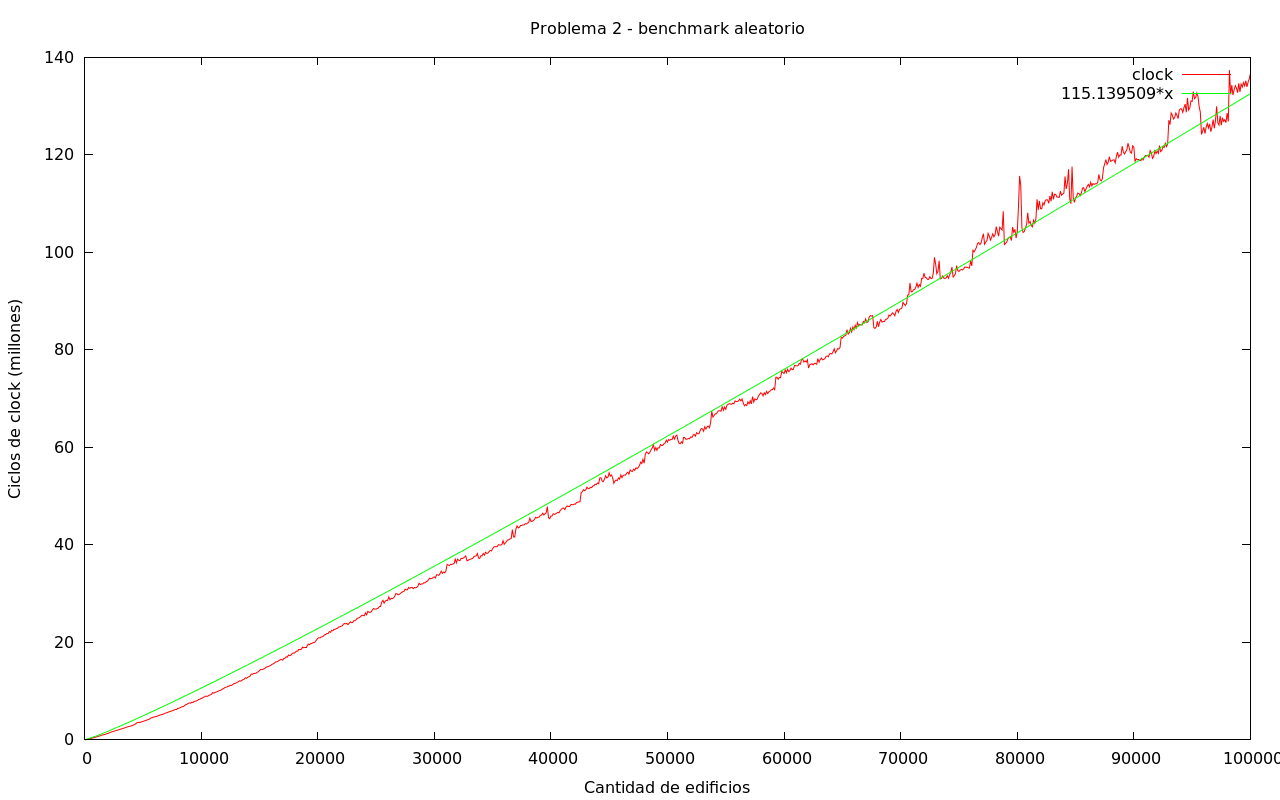
\includegraphics[scale=0.35]{imagenes/grafico-2.png}
  \end{center}
\end{figure}

\vspace*{0.5cm}

En este gráfico podemos apreciar que, los valores que toma la curva que representa la cantidad de ciclos
de clock empieza tomando valores \textbf{menores} a nuestra curva de referencia, para después \textbf{acercarse} bastante \textbf{y
luego superarla}, tal como se comportaría una curva del estilo $y = x \log x$, pero en este caso está más
"linealizada" por tratarse del caso aleatorio.

\newpage


\subsubsection{Test 2 - benchmark del peor caso}

(ver \verb|info.2.peor.dat|) \medskip

En este test, $n$ (cantidad de edificios) se inicializa en 100 y va incrementándose también de a 100,
hasta alcanzar 100000. Tomamos como peor caso, una instancia en la cual se generan alturas de 1 a $n$,
se mezclan y luego se generan paredes que van "achicándose", es decir, para la primer altura tenemos
\verb|1 2n|, para la segunda \verb|2 2n-1| y así sucesivamente.

Para cada instancia, se toma el \textbf{valor mínimo} de cantidad de ciclos luego de \textbf{25 corridas}.

\vspace*{0.5cm}

\begin{figure}[h]
  \begin{center}
    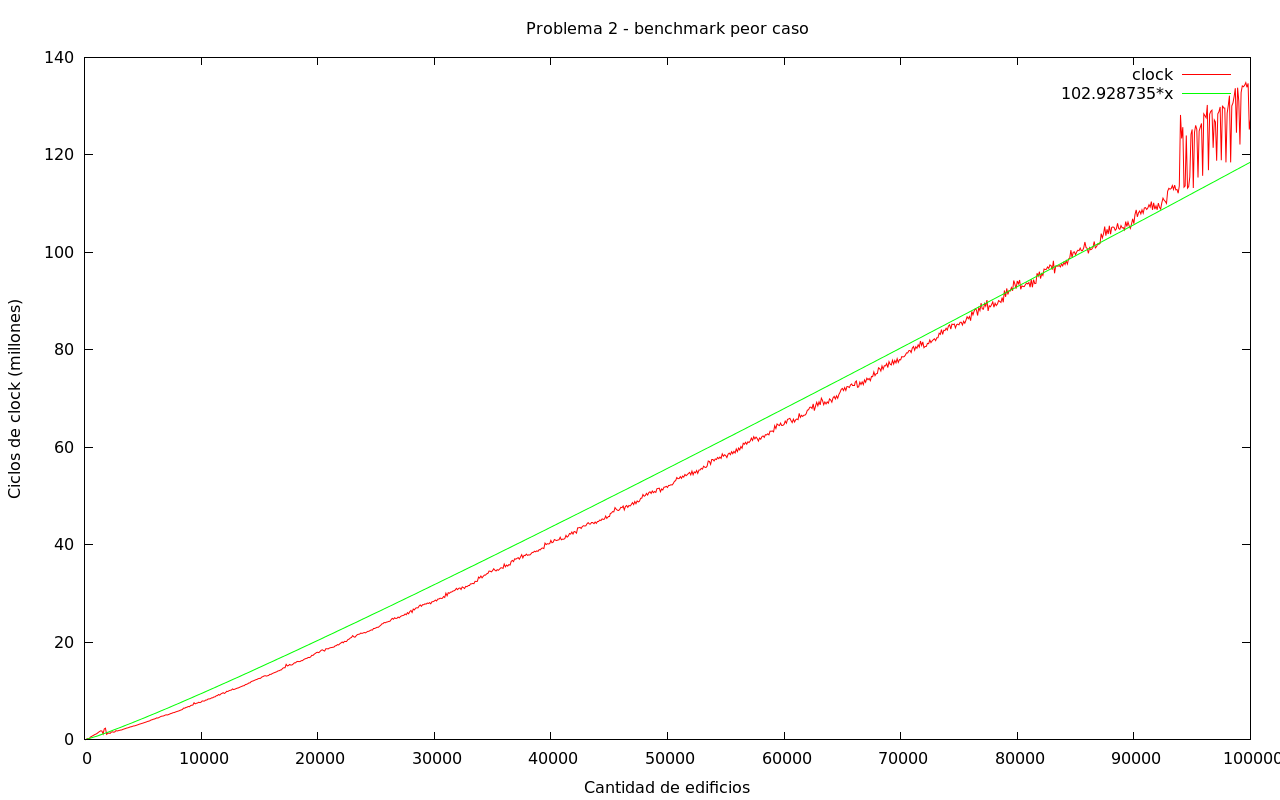
\includegraphics[scale=0.35]{imagenes/grafico-2-peor.png}
  \end{center}
\end{figure}

\vspace*{0.5cm}

En este gráfico podemos apreciar que, al igual que en el experimento aleatorio, los valores que toma la curva
que representa la cantidad de ciclos de clock empieza tomando valores menores a nuestra curva de referencia,
para después acercarse bastante y luego superarla, tal como se comportaría una curva del estilo $y = x*log(x)$,
pero, a diferencia del anterior, en el punto donde la curva de referencia es superada, \textbf{la curva que mide nuestro
algoritmo crece a mayor velocidad} . Para $n$ = 90000 aproximadamente, la curva de referencia ya se ve superada,
mientras que en el experimento aleatorio se mantenían en valores similares.


\newpage


\subsubsection{Test 3 - benchmark del mejor caso}

(ver \verb|info.2.mejor.dat|) \medskip

En este test, $n$ (cantidad de edificios) se inicializa en 100 y va incrementándose también de a 100,
hasta alcanzar 100000. Tomamos como mejor caso una instancia con un \textit{gran edificio}, que posee dentro
edificios disjuntos (es decir, cuyas paredes no se instersectan).

Para cada instancia, se toma el \textbf{valor mínimo} de cantidad de ciclos luego de \textbf{25 corridas}.


\begin{figure}[h]
  \begin{center}
    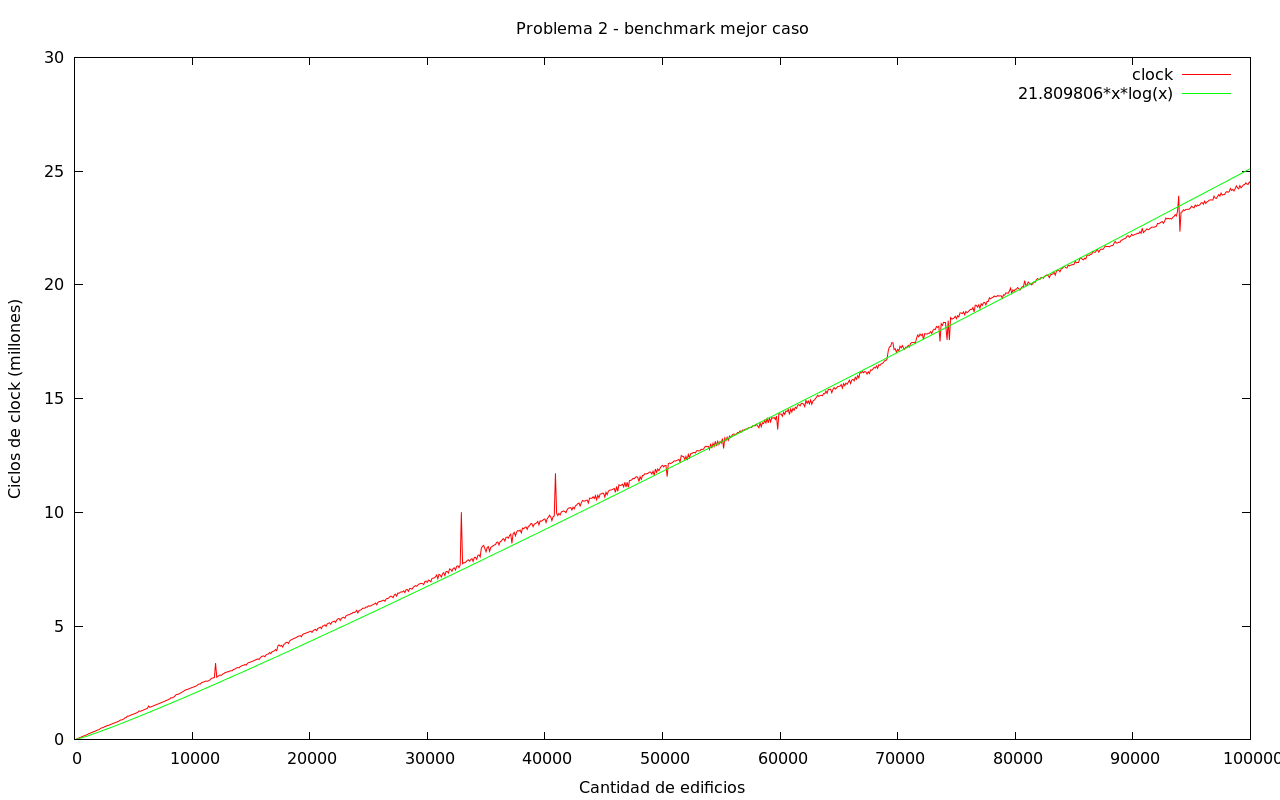
\includegraphics[scale=0.35]{imagenes/grafico-2-mejor.png}
  \end{center}
\end{figure}


En este gráfico podemos apreciar que, a diferencia de los dos experimentos anteriores, el comportamiento
del algoritmo es \textbf{prácticamente lineal}, reduciendo además la cantidad de ciclos requeridos hasta un 75\%
aproximadamente. También es importante notar que la curva que representa los valores en ciclos requeridos
por nuestro algoritmo \textbf{se mantiene acotada superiormente por la curva tomada de referencia}. Entendemos que
para aquellos puntos donde sí la supera, se debe más bien a errores en la medición o momentos de sobrecarga
del procesador, que influyen en el resultado del experimento.
